\documentclass[../main.tex]{subfiles}
\graphicspath{{../images/}}

\begin{document}
\subsection*{Lecture 9: \hfill  2/5/24}
\hrule \vspace{10px}
\section{Oscillations}

\& Simple Harmonic Oscillators For the simple case of a mas on a spring, the spring force is
$F_{s} = -k(x - x_o)$
where the force is conservative and the (elastic) potential energy is
$U_s = \frac{1}{2} k (x - x_o)^2$.

\paragraph*{Aribtrary Potential energy} 
% insert fig
\begin{figure}[ht]
    \centering
    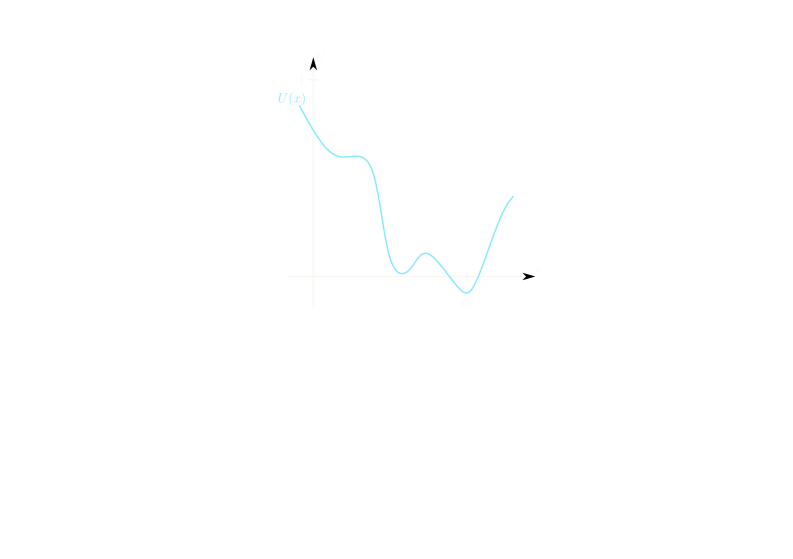
\includegraphics[width=0.5\textwidth]{5_1.png}
    \caption{Arbitrary Potential Energy: $\vb{F} = - \grad U$}
    \label{fig:fig1}
\end{figure}

For a equilibrium positon $x_o$ we can take the taylor expansion of the potential energy
\begin{align*}
    U(x) = U(x_o) + U' (x_o) \Delta x + \frac{1}{2} U''(x_o) \Delta x^2 + \dots
\end{align*}
where $\Delta x = x - x_o$. Setting $x_o$ to the reference point of $U$ cancels the first term and
the conservative nature tells us that the second term is also zero thus we are left with the third
term where the spring constant is
\begin{align*}
    k = U'' (x_o)
\end{align*}
To find the equations of motion, using N2L
\begin{align*}
    m\ddot x &= F = - k (x - x_o) \\
    \ddot x &= - \frac{k}{m} (x - x_o)
\end{align*}
where we have a constant of angular frequency
\begin{align*}
    \omega_o = \sqrt{\frac{k}{m}}
\end{align*}
the solution could be a sinusoidal function
\begin{align*}
    x(t) \approx \sin \omega_o t 
\end{align*}
but we are missing the initial value, so
\begin{align*}
    x(t) \approx \sin \omega_o t + x_o
\end{align*}
the general solution is linear combinations of the sine and cosine functions
\begin{align*}
    x(t) &= A \sin \omega_o t + B \cos \omega_o t + x_o \\
    \dot x(t) &= \omega_o A \cos \omega_o t - \omega_o B \sin \omega_o t
\end{align*}
where we need 2 initial conditions to solve for $A$ and $B$. e.g. $x(0)$ and $\dot x(0)$.
\begin{align*}
    B &= x(0) - x_o = \Delta x(0), \qquad A = \frac{\dot x(0)}{\omega_o}
\end{align*}

\paragraph*{Euler's Solution} We can also use a general solution of the form
\begin{align*}
    e^{i \theta} = \cos \theta + i \sin \theta
\end{align*}
where
\begin{align*}
    \abs {e^{i \theta}} = \cos^2 \theta + \sin^2 \theta = 1
\end{align*}
taking the derivatives
\begin{align*}
    \dv{t} e^{i \omega_o t} &= i \omega_o e^{i \omega_o t} \\
    \dv[2]{t} e^{i \omega_o t} &= - \omega_o^2 e^{i \omega_o t}
\end{align*}
and the general solution is
\begin{align*}
    x(t) &= A e^{i \omega_o t} + B e^{-i \omega_o t} + x_o
\end{align*}
this does not mean that we have an imaginary solution, but rather we are using the geomtric 
nature of the solution. 

\paragraph*{Third Way} We can also use a method where we introduce the phase
\begin{align*}
    x(t) &= A \cos(\omega_o t - \delta) + x_o \\
    \dot x(t) &= -A \omega_o \sin(\omega_o t - \delta)
\end{align*}
for $t = 0$ we have
\begin{align*}
    x(0) &= A \cos(-\delta) + x_o = A \cos \delta + x_o \\
    \dot x(0) &= -A \omega_o \sin(-\delta) = A \omega_o \sin \delta
\end{align*}
and the constants are found by squaring and adding the two equations
\begin{align*}
    A^2 &= (x(0) - x_o)^2 + \frac{\dot x(0)^2}{\omega_o^2}
        = \Delta x(0)^2 + \frac{\dot x(0)^2}{\omega_o^2}\\
    \delta &= \arctan \frac{\dot x(0)}{\omega_o (x(0) - x_o)}
        = \arctan \frac{\dot x(0)}{\omega_o \Delta x(0)}
\end{align*}

\paragraph*{Energy of the Oscillator} The mechanical energy is $E = T + U$
\begin{align*}
    T &= \frac{1}{2} m \dot x^2 = \frac{1}{2} m \omega_o^2 A^2 \sin^2(\omega_o t - \delta) \\
    U &= \frac{1}{2} k (x - x_o)^2 = \frac{1}{2} k A^2 \cos^2(\omega_o t - \delta)
\end{align*}
setting $x_o = 0$ we can work with a much simple case
\begin{align*}
    U &= \frac{1}{2} k x^2 \\  
    T &= \frac{1}{2} k x^2
\end{align*}
using the third way where
\begin{align*}
    x(t) &= A \cos(\omega_o t - \delta) \\
    \dot x(t) &= -A \omega_o \sin(\omega_o t - \delta)
\end{align*}
we have
\begin{align*}
    U &= \frac{1}{2} k x^2 = \frac{1}{2} k A^2 \cos^2(\omega_o t - \delta) \\
    T &= \frac{1}{2} m \dot x^2 = \frac{1}{2} m A^2 \omega_o^2 \sin^2(\omega_o t - \delta)
    &= \frac{1}{2} k A^2 \sin^2(\omega_o t - \delta)
\end{align*}
thus the total mechanical energy is
\begin{align*}
    E = T + U = \frac{1}{2} k A^2
\end{align*}
where this is the maximum potential energy of the system, or the potential energy at the maximum 
amplitude. This is also the classical turning point $E = U$. As time goes on, we can see that the
energy oscillates betweeen being completely kinetic $(T)$ and completely potential $(U)$.

\paragraph*{2D Oscillator} We can have two cases of oscillation:
\begin{align*}
    \vb{F} = -k (\vb{r} - \vb{r}_o) \quad \textrm{isotropic oscillator}
\end{align*}
this is where each component share the same frequency, but different amplitudes and/or initial
conditions
\begin{align*}
    x(t) &= A_x \cos(\omega_o t - \delta_x) + x_o \\
    y(t) &= A_y \cos(\omega_o t - \delta_y) + y_o
\end{align*}
for the anisotropic oscillator
\begin{align*}
    F_x &= -k_x (x - x_o) \quad F_y = -k_y (y - y_o)
\end{align*}
the frequency is decoupled thus
\begin{align*}
    x(t) &= A_x \cos(\omega_{ox} t - \delta_x) + x_o \\
    y(t) &= A_y \cos(\omega_{oy} t - \delta_y) + y_o
\end{align*}
and if the ratio between the angular frequencies $\omega_{ox} / \omega_{oy}$ are rational, the
motion is periodic and the figure will be closed. But for irrational ratios, the motion is
\emph{quasiperiodic} and the figure is not closed (chaotic).

\newpage
\subsection*{Lecture 10: \hfill  2/7/24}
\hrule \vspace{10px}

\section*{Oscillations: Damping}

\paragraph{Damped Oscillator} From last time the simple EOM for a spring is
\begin{align*}
    m \ddot x = - k (x - x_o)
\end{align*}
where the equilibrium position is $x_o$ and the spring constant is $k$. When we add air resistance
e.g. linear drag:
\begin{align*} 
    \vb{f} = -b \vb{v} \qquad m\ddot x = -kx - b \dot x
\end{align*}
or
\begin{align*}
    \ddot x + \frac{b}{m} \dot x + \frac{k}{m} x = 0
\end{align*}
where we have two constants
\begin{align*}
    \omega_o = \sqrt{\frac{k}{m}} \quad \beta = \frac{b}{2m}
\end{align*}
where $\omega_o$ is the natural frequency and $\beta$ is the damping coefficient. Rewriting in terms
of the constants we get
\begin{align*}
    \ddot x + 2 \beta \dot x + \omega_o^2 x = 0
\end{align*}
where a general solution is
\begin{align*}
    x = e^{rt}; \quad \dot x = r e^{rt}; \quad \dot x = r^2 e^{rt}
\end{align*}
plugging into the EOM gives
\begin{align*}
    r^2 e^{rt} + 2 \beta r e^{rt} + \omega_o^2 e^{rt} = 0 \\
    r^2 + 2 \beta r + \omega_o^2 = 0
\end{align*}
which is the characteristic (or auxiliary) equation, and the solution is in the form of 
the quadratic formula
\begin{align*}
    r_{1,2} = -\beta \pm \sqrt{\beta^2 - \omega_o^2}
\end{align*}
thus the position is a linear combination of the two solutions
\begin{align*}
    x(t) = C_1 e^{(-\beta + \sqrt{\beta^2 - \omega_o^2}) t} 
        + C_2 e^{(-\beta - \sqrt{\beta^2 - \omega_o^2}) t}
\end{align*}
At $\beta = 0$ (no damping)
\begin{align*}
    \sqrt{\beta^2 - \omega_o^2} = \sqrt{-\omega_o^2} = i \omega
\end{align*}
thus the solution of a SHO
\begin{align*}
    x(t) = C_1 \exp(i \omega t) + C_2 \exp(-i \omega t)
\end{align*}

\paragraph*{Weak Damping}
For the case $\beta < \omega_o$ (underdamping)
\begin{align*}
    \sqrt{\beta^2 - \omega_o^2} = i \sqrt{\omega_o^2 - \beta^2}
\end{align*}
thus the solution is
\begin{align*}
    x(t) &= C_1 e^{(-\beta + i \sqrt{\omega_o^2 - \beta^2}) t} + C_2 e^{(-\beta - i \sqrt{\omega_o^2 - \beta^2}) t} \\
    &= e^{-\beta t} (C_1 \cos(\sqrt{\omega_o^2 - \beta^2} t) + C_2 \sin(\sqrt{\omega_o^2 - \beta^2} t))
\end{align*}
we can simplify this with a new frequency term $\omega_1 = \sqrt{\omega_o^2 - \beta^2}$ and
therefore
\begin{align*}
    x(t) = A e^{-\beta t} \cos(\omega_1 t - \delta)
\end{align*}
this is called underdamping because the amplitude oscillates and decays slowly. 

\paragraph*{Strong damping}
For the case $\beta > \omega_o$ we have the solution
\begin{align*}
    x(t) = e^{-(\beta - \sqrt{\beta^2 - \omega_o^2})t} \qt(C_1 + C_2 e^{-2\sqrt{\beta^2 - \omega_o^2} t})
\end{align*}
this called overdamping because the system cannot cannot complete a full oscillation, and decays
exponentially to the equilibrium position. Thus we call the term
\begin{align*}
    \textrm{decay parameter} = \beta - \sqrt{\beta^2 - \omega_o^2}
\end{align*}
where the decaying tail is described by the decay parameter whereas the second term
$-2\sqrt{\beta^2 - \omega_o^2}$ describes the fast initial damping of the system.

\paragraph*{Large $\beta$} For the case of $\beta \to \infty$ the decay parameter goes to zero:
\begin{align*}
    \gamma = \beta - \sqrt{\beta^2 - \omega_o^2} \to 0
\end{align*}
which is counter intuitive as the high damping coefficient results in a very slow exponential decay
where it looks like a constant almost zero.

\paragraph*{Critical Damping} For the case $\beta = \omega_o$ we get
\begin{align*}
    x(t) = C_1 e^{-\beta t} + C_2 t e^{-\beta t} \to x = e^{-\beta t}(C_1 + C_2 t)
\end{align*}
where the extra factor of $t$ comes from solving for a function $f(t)e^{-\beta t}$ to get the 
Constants. Pluggin this back into the initial EOM: $\ddot x + 2 \beta \dot x + \omega_o^2 x = 0$
\begin{align*}
    \dot x = e^{-\beta t} - t e^{-\beta t} \qquad \ddot x = -2 \beta e^{-\beta t} + t e^{-\beta t}
\end{align*}
so
\begin{align*}
    -2\beta e^{-\beta t} + \beta^2 t e^{-\beta t} + 2 \beta e^{-\beta t} - 2\beta^2 t e^{-\beta t} 
    + \beta^2 t e^{-\beta t} = 0
\end{align*}
% 2x4 table 
\begin{center}
    \begin{tabular}{c | c}
        condition & $\gamma$ \\
        \hline
        $\beta < \omega_o$ & $\beta$ \\
        $\beta = \omega_o$ & $\beta$ \\
        $\beta > \omega_o$ & $\beta - \sqrt{\beta^2 - \omega_o^2} $\\        
    \end{tabular}
\end{center}
the critical damping will have the fastest decay of the system. The quickest way to stop an
oscillating system is to apply a damping force at the natural frequency of the system.

\paragraph*{NOTE:} This all goes away when the magnitude of the damping force is not linear (e.g.
quadratic drag). The linear EOM gives us something that can be easily analyzed, but for terms with
higher powers (e.g. $\dot x^2$) the EOM becomes non-linear and the solutions are chaotic.

\newpage
\subsection*{Lecture 11: \hfill  2/9/24}
\hrule \vspace{10px}

\section*{Driven Damped Oscillations}
\paragraph*{From last time:} Note that the two parameters $\omega_o$ and $\beta$ have the same units
($\unit{\radian/\s}$) where we treat radians as a unitless quantity. 

\paragraph*{Time dependent force} For the SHO we have a new EOM
\begin{align*}
    m \ddot x + b \dot x + kx = F \cos(\omega t)
\end{align*}
or in terms of the constants $\omega_o$ and $\beta$
\begin{align*}
    \ddot x + 2 \beta \dot x + \omega_o^2 x = \frac{F(t)}{m} = f(t) 
\end{align*}
where $f(t)$ has the same units as acceleration/ force per unit mass. This is a inhomogeneous
differential equation, but we can consider this as a combination of a homogeneous solution $x_h$ and
a particular solution $x_p$:
\begin{align*}
    x_p(t) + x_h(t) = x(t)
\end{align*}
denoting a differential operator
\begin{align*}
    D = \dv[2]{t} + 2 \beta \dv{t} + \omega_o^2
\end{align*}
we know that
\begin{align*}
    D x_h(t) = 0 \qquad D x_p(t) = f(t)
\end{align*}
where from last time we know that the homogeneous solution is
\begin{align*}
    x_h(t) = e^{-\beta t} (C_1 \exp(t\sqrt{\beta^2 - \omega_o^2})
        + C_2 \exp(-t\sqrt{\beta^2 - \omega_o^2}))
\end{align*}
and for the particular solution we can define the driving force as a sinusoidal function
\begin{align*}
    f(t) = f_o \cos(\omega t) \qqtext{driving force}
\end{align*}
where
\begin{align*}
    \ddot x + 2\beta \dot x + \omega_o^2 x = f_o \cos \omega t
\end{align*}
or using Euler's formula we can define the EOM as the real part of the complex function
\begin{align*}
    \ddot x + 2\beta \dot x + \omega_o^2 x = f_o e^{i \omega t}
\end{align*}
the particular solution is then
\begin{align*}
    x = C e^{i \omega t} \\
    \dot x = i \omega C e^{i \omega t}, \qquad \ddot x = -\omega^2 C e^{i \omega t}
\end{align*}
subbing this back in to the EOM
\begin{align*}
    -\omega^2 C e^{i \omega t} + 2 \beta i \omega C e^{i \omega t} + \omega_o^2 C e^{i \omega t} 
    = f_o e^{i \omega t}
\end{align*}
or 
\begin{align*}
    C = \frac{f_o}{\omega_o^2 - \omega^2 + 2 i \beta \omega}
\end{align*}
which is a complex number. Before taking the real part of the solution,
\begin{align*}
    x(t) = \Re(C e^{i \omega t})
\end{align*}
we have to consider the complex part as well, so we rewrite $C$ as
\begin{align*}
    C = A e^{-i\delta} = A \cos \delta - i A \sin \delta
\end{align*}
so the real part of the solution is
\begin{align*}
    x(t) = \Re (A e^{i(\omega t - \delta)}) = A \cos(\omega t - \delta)
\end{align*}
to find the amplitude $A$ we have to multiply $C$ by its complex conjugate
\begin{align*}
    C^* C = \abs{C}^2 = A^2
\end{align*}
where we get the modulus squared. Thus we get
\begin{align*}
    A^2 = \frac{f_o^2}{(\omega_o^2 - \omega^2)^2 + (2\beta \omega)^2}
\end{align*}
to find $\delta$ we move some terms around 
\begin{align*}
    \frac{f_o}{\omega_o^2 - \omega^2 + 2 i \beta \omega} &= A e^{-i \delta} \\
    f_o e^{i\delta} &= A(\omega_o^2 - \omega^2 + 2 i \beta \omega) \\
    f_o \cos \delta + i f_o \sin \delta &= A(\omega_o^2 - \omega^2 + 2 i \beta \omega)
\end{align*}
thus we have
\begin{align*}
    \sin \delta &= \frac{2 A \beta \omega}{f_o} \qquad 
    \cos \delta = \frac{A(\omega_o^2 - \omega^2)}{f_o} \\
\end{align*}
dividing the two equations gives us the phase
\begin{align*}
    \delta = \arctan(\frac{2\beta \omega}{\omega_o^2 - \omega^2})
\end{align*}

\pagebreak
The full solution is now
\begin{align*}
    x(t) &= x_p(t) + x_h(t) \\
        &= A \cos(\omega t - \delta) +  C_1 e^{\qt(-\beta  + \sqrt{\beta^2 - \omega_o^2})t}
        +  C_2 e^{\qt(-\beta  - \sqrt{\beta^2 - \omega_o^2})t}
\end{align*}
where $\omega$ is the driving frequency, and $\omega_o$ is the natural frequency. The last two 
exponential terms are known as the transient solution which decays very quick (exponentially) as
shown in Figure \ref{fig:transientsolution}
\begin{figure}[ht]
    \centering
    \includegraphics[width=0.4\textwidth]{transient.png}
    \caption{Driven Damped Oscillations}
    \label{fig:transientsolution}
\end{figure}
Finding the maximum we look for where the derivative of $A^2$ is zero, or roughly
\begin{align*}
    \dv{\omega} \qt((\omega_o^2 - \omega^2)^2 + (2\beta \omega)^2) = 0
\end{align*}
which gives us
\begin{align*}
    \omega = \omega_2 = \sqrt{\omega_o^2 - 2\beta^2}
\end{align*}

where at $B \ll \omega_o \to \omega \approx \omega_o$. Figure \ref{fig:resonance} shows that
$\omega_2$ is a resonant frequency where the amplitude is maximized.
\begin{align*}
    A_{max} = \frac{f_o}{\sqrt{4\beta^2 (\omega_o^2 - \omega^2)}} \approx \frac{f_o}{2\beta \omega}
    \qqtext{for} \beta \ll \omega_o
\end{align*}

\begin{figure}
    \centering
    \begin{minipage}{0.5\textwidth}
        \centering
        \includegraphics[width=0.8\textwidth]{amplitude.png}
        \caption{Resonance at $\omega_2$}
        \label{fig:resonance}
        \end{minipage}%
    \begin{minipage}{0.5\textwidth}
        \centering
        \includegraphics[width=0.8\textwidth]{delta.png}
        \caption{Phase shift $\delta$}
        \label{fig:phase}    
    \end{minipage} 
\end{figure}
\paragraph*{What is $\delta$?} From the general solution, we can see that $\delta$ is a shift with
respect to the driving force. This lag we can graph as a function of $\omega$ as shown in Figure
\ref{fig:phase}


\end{document}